\documentclass[10pt,twocolumn,letterpaper]{article}
\usepackage{fontspec}
\setmainfont{TeX Gyre Termes}
\usepackage{polyglossia}
\setdefaultlanguage{spanish}
\usepackage[top=0.75in,bottom=1in,left=0.625in,right=0.625in,columnsep=0.25in]{geometry}
\usepackage{amsmath,amssymb}
\usepackage{graphicx}
\usepackage{booktabs}
\usepackage{stfloats}
\usepackage{cite}
\usepackage[font=footnotesize,labelsep=period]{caption}
\usepackage{titlesec}
\usepackage[hidelinks]{hyperref}

\graphicspath{{../figures/}}
\renewcommand{\thesection}{\Roman{section}}
\renewcommand{\thesubsection}{\Alph{subsection}}
\titleformat{\section}{\normalfont\scshape\centering}{\thesection.}{0.5em}{}
\titleformat{\subsection}{\normalfont\itshape}{\thesubsection.}{0.5em}{}
\titlespacing*{\section}{0pt}{1.1ex}{0.7ex}
\titlespacing*{\subsection}{0pt}{0.9ex}{0.4ex}
\captionsetup[figure]{name=Fig.}
\captionsetup[table]{name=TABLA,labelfont=sc,justification=centering}
\renewcommand{\thetable}{\Roman{table}}
\setlength{\parindent}{1em}
\setlength{\parskip}{0pt}
\pagestyle{plain}

\begin{document}

\twocolumn[
\begin{center}
{\LARGE Más datos en el mismo canal: comparación de QPSK y 16QAM con igual tasa de símbolos en GNU Radio y HackRF One\par}
\vspace{0.9em}
{\large Nicolas Alvarez Alvarez (2192317), Karoll Juliana Ruiz Martinez (2224724)\\ y Liliam Daniela Rodriguez Morales (2192316)\par}
\vspace{0.3em}
{\small\itshape Comunicaciones II (27145), Grupo 3 · Escuela de Ingenierías Eléctrica, Electrónica y de Telecomunicaciones\\
Universidad Industrial de Santander, Bucaramanga, Colombia · Noviembre de 2026\par}
\vspace{1em}
\begin{minipage}{0.92\textwidth}
\small\bfseries\itshape Resumen---\normalfont\bfseries
Cuando un enlace necesita transportar más información pero tiene asignado un canal de ancho fijo, no se puede aumentar la tasa de símbolos. La alternativa es enviar más bits en cada símbolo. En este trabajo se compararon QPSK y 16QAM con la misma tasa de símbolos ($R_s=32$~ksym/s), las mismas muestras por símbolo ($S_{ps}=8$) y la misma tasa de muestreo ($f_s=256$~kS/s), usando los flujogramas del curso en GNU Radio y un único nivel de ruido AWGN que se varió en cuatro pruebas. Las dos modulaciones ocuparon el mismo ancho de banda, pero 16QAM entregó 128~kb/s frente a 64~kb/s de QPSK. El precio fue la robustez: con energía promedio normalizada, la distancia mínima de 16QAM es 0.63 frente a 1.41 de QPSK, y en la prueba de ruido fuerte 16QAM tuvo una BER de $4.2\times10^{-3}$, mientras que QPSK no tuvo errores. Por teoría, 16QAM necesita unos 3.7~dB más de $E_b/N_0$ para alcanzar una BER de $10^{-3}$. Finalmente, el enlace 16QAM se llevó a hardware con dos HackRF One a 960~MHz, donde se recuperaron tramas con una BER cercana al 0.34\,\%.
\par\vspace{0.5em}
\small\bfseries\itshape Palabras clave---\normalfont\bfseries QPSK, 16QAM, AWGN, eficiencia espectral, GNU Radio, SDR, BER.
\end{minipage}
\vspace{1.4em}
\end{center}
]

\section{Introducción}
En muchas plantas industriales los datos de inspección (imágenes de una cámara, medidas de sensores o estados de máquinas) viajan por enlaces inalámbricos hasta una sala de control. Con el tiempo, estas aplicaciones suelen pedir más información: más resolución, más variables o mayor frecuencia de actualización. El problema es que el espectro asignado normalmente no crece al mismo ritmo, y el canal sigue teniendo el mismo ancho.

El escenario S4 del proyecto \cite{guia} plantea justamente esta situación: transportar más bits sin aumentar de manera importante la tasa de símbolos. Como el ancho de banda depende de $R_s$ y no del número de puntos de la constelación, la salida natural es pasar de una modulación de 2 bits por símbolo (QPSK) a una de 4 bits por símbolo (16QAM). Este paso no es gratis. Al poner más puntos en el mismo plano, con la misma potencia, los puntos quedan más cerca y el ruido los confunde con más facilidad \cite{proakis,sklar}. Los sistemas reales manejan este compromiso con modulación adaptativa: usan 16QAM o más cuando el enlace es bueno y regresan a QPSK cuando empeora \cite{goldsmith}.

El objetivo de este trabajo fue mostrar ese compromiso de forma medible. Se simularon las dos modulaciones en GNU Radio con los mismos parámetros, se varió solo el nivel de ruido y se observaron la PSD, la constelación y la señal en el tiempo. Además, se calculó la tasa de error y se validó el enlace 16QAM en hardware con dos radios HackRF One. La Fig.~\ref{fig:escenario} muestra el escenario que se tomó como referencia.

\begin{figure*}[!t]
\centering
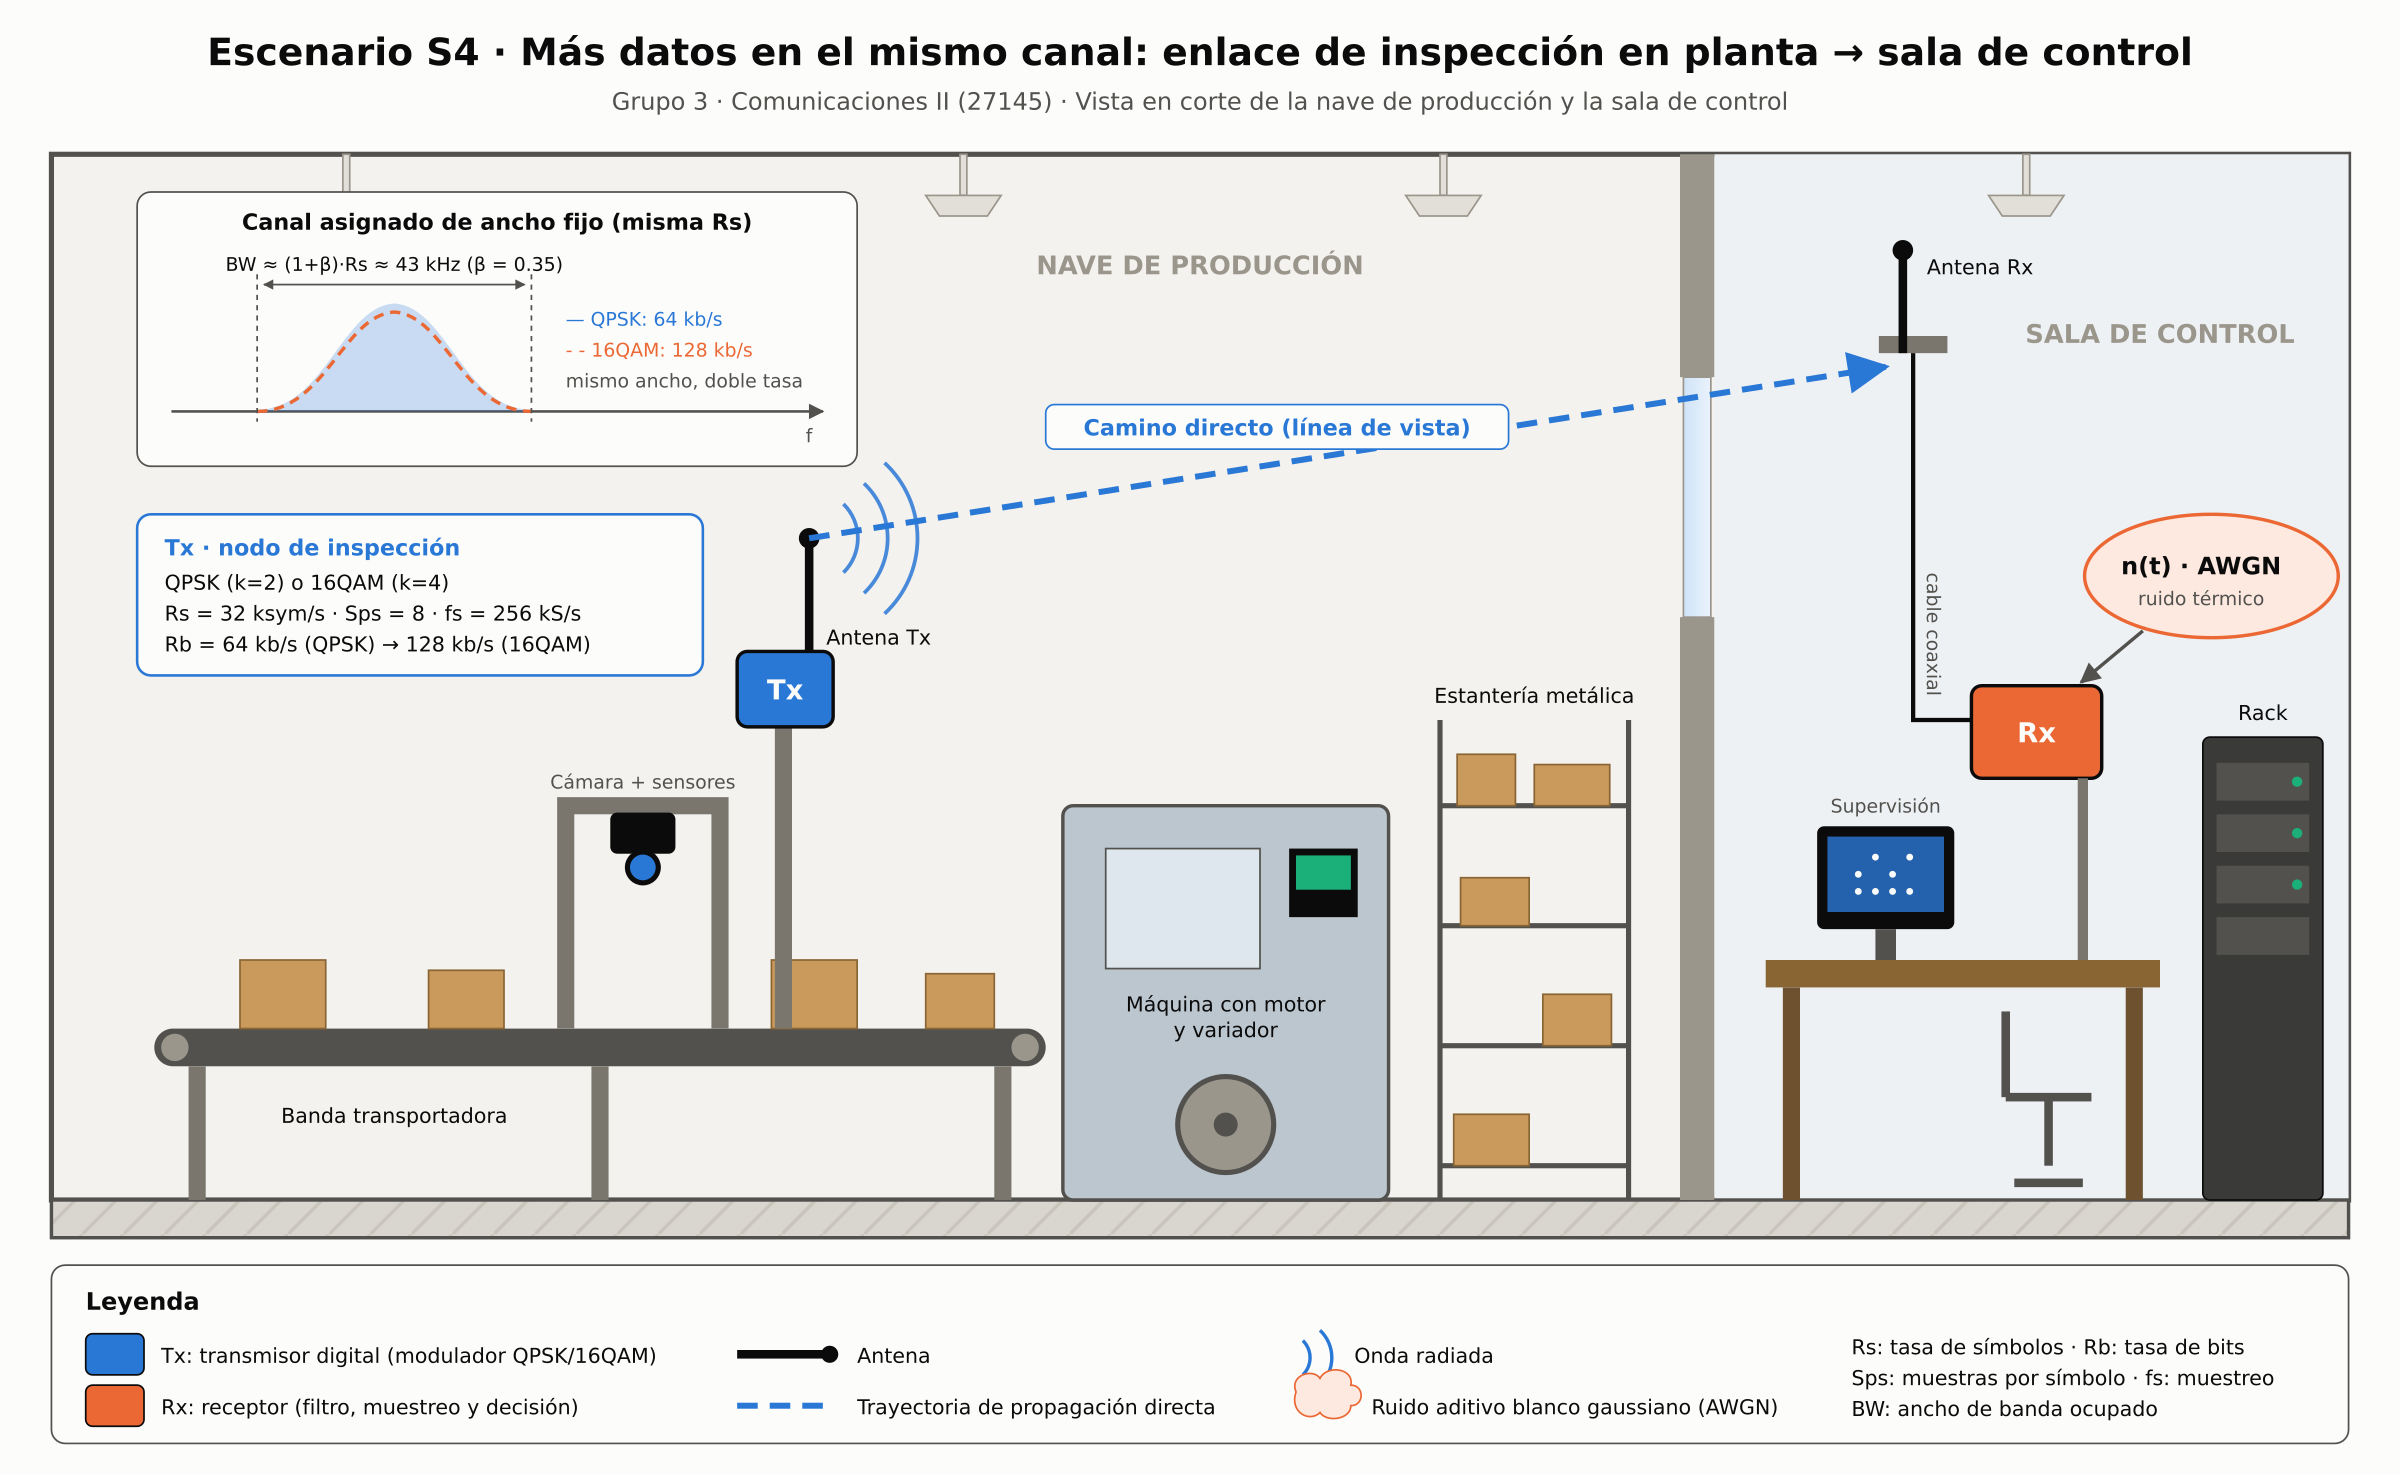
\includegraphics[width=0.93\textwidth]{escenario/fig1_escenario_contextual.png}
\caption{Escenario contextual. Un nodo de inspección (Tx) sobre la banda transportadora envía datos a la sala de control (Rx) por un canal de ancho fijo. La principal perturbación es el ruido térmico en el receptor, modelado como AWGN.}
\label{fig:escenario}
\end{figure*}

\section{Fundamento teórico}
\subsection{Bits por símbolo, tasas y ancho de banda}
Una modulación de $M$ símbolos transporta $k=\log_2 M$ bits por símbolo, de modo que
\begin{equation}
R_b = R_s\,k, \qquad f_s = R_s\,S_{ps}.
\end{equation}
Para QPSK $k=2$ y para 16QAM $k=4$. El ancho de banda ocupado depende de la forma del pulso y de $R_s$. Con pulso rectangular, el lóbulo principal de la PSD mide $2R_s$, con nulos en $\pm R_s$. Con un filtro de raíz de coseno alzado (RRC) de factor $\beta$, se aproxima a
\begin{equation}
BW \approx (1+\beta)\,R_s.
\end{equation}
Si $R_s$ y el pulso se mantienen, el ancho de banda es el mismo para las dos modulaciones. Por eso la eficiencia espectral $R_b/BW$ de 16QAM es el doble de la de QPSK.

\subsection{Normalización de energía y distancia mínima}
Para comparar las dos modulaciones de forma justa, ambas deben transmitir la misma energía promedio por símbolo, $E_s=1$. La constelación QPSK usada, $\{1, j, -j, -1\}$, ya cumple esta condición. En cambio, los puntos de 16QAM $\{\pm1,\pm3\}\pm j\{\pm1,\pm3\}$ tienen energía promedio 10, y por eso se dividen entre $\sqrt{10}$. Con esta normalización, la distancia mínima entre puntos vecinos queda en
\begin{equation}
d_{\min}^{\text{QPSK}}=\sqrt{2}\approx1.41,\qquad d_{\min}^{\text{16QAM}}=\tfrac{2}{\sqrt{10}}\approx0.63.
\end{equation}
Los puntos de 16QAM están 2.2 veces más cerca, y esa es la razón física de su menor robustez (Fig.~\ref{fig:ideales}). Además, se usó codificación Gray en 16QAM, de modo que dos símbolos vecinos solo difieren en un bit.

\begin{figure}[!t]
\centering
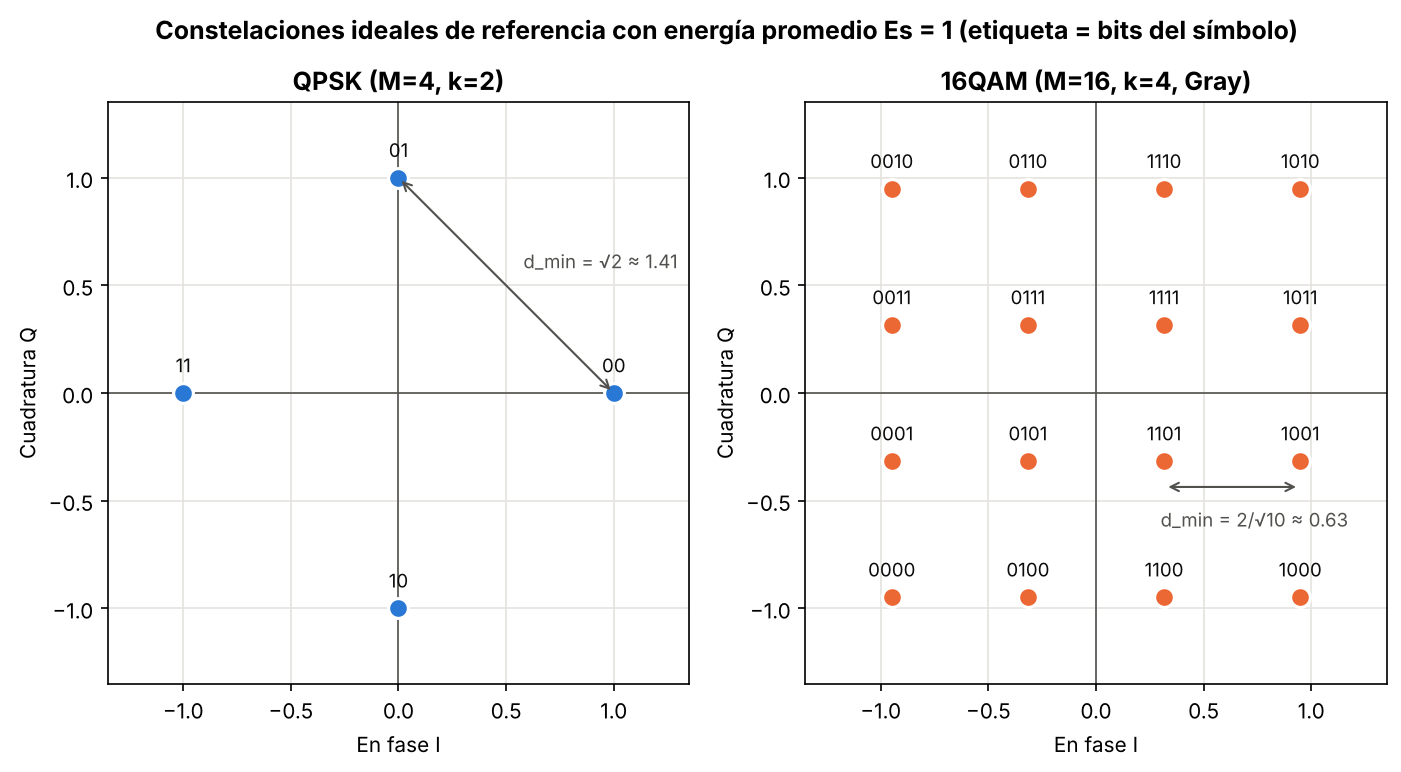
\includegraphics[width=\columnwidth]{diagramas_tecnicos/fig_constelaciones_ideales_QPSK_16QAM.png}
\caption{Constelaciones ideales de referencia con $E_s=1$. Cada punto lleva la etiqueta de los bits que representa.}
\label{fig:ideales}
\end{figure}

\subsection{Ruido AWGN y probabilidad de error}
El ruido térmico se modela como ruido aditivo blanco gaussiano (AWGN) \cite{haykin}. En un canal AWGN, con filtro acoplado y codificación Gray, la tasa de error de bit es aproximadamente \cite{proakis}
\begin{align}
P_b^{\text{QPSK}} &= Q\!\left(\sqrt{2E_b/N_0}\right),\\
P_b^{\text{16QAM}} &\approx \tfrac{3}{4}\,Q\!\left(\sqrt{\tfrac{4}{5}E_b/N_0}\right).
\end{align}
Para una BER de $10^{-3}$, QPSK necesita $E_b/N_0\approx6.8$~dB y 16QAM unos 10.5~dB. La diferencia, cercana a 3.7~dB, es el costo de duplicar la tasa de bits.

\section{Diseño del sistema y parámetros}
Se partió de los parámetros del paquete A de la ficha de decisión técnica, que se mantuvieron fijos en todas las pruebas (Tabla~\ref{tab:param}). Se verificó que $f_s=R_s\,S_{ps}=32\,000\times8=256\,000$~muestras/s coincide con \texttt{samp\_rate} del flujograma.

\begin{table}[!t]
\caption{Parámetros del sistema simulado}
\label{tab:param}
\centering\small
\begin{tabular}{@{}lcc@{}}
\toprule
Parámetro & QPSK & 16QAM\\
\midrule
$M$ / $k$ & 4 / 2 & 16 / 4\\
$R_s$ & 32 ksym/s & 32 ksym/s\\
$R_b=R_s k$ & \textbf{64 kb/s} & \textbf{128 kb/s}\\
$S_{ps}$ / $f_s$ & 8 / 256 kS/s & 8 / 256 kS/s\\
BW (rect., $2R_s$) & 64 kHz & 64 kHz\\
BW (RRC, $\beta=0.35$) & 43.2 kHz & 43.2 kHz\\
$R_b/BW$ (RRC) & 1.5 b/s/Hz & 3.0 b/s/Hz\\
\bottomrule
\end{tabular}
\end{table}

La Fig.~\ref{fig:bloques} muestra la cadena completa. Una fuente aleatoria entrega bits que se agrupan de a $k$ (\emph{Pack K Bits} y \emph{Unpack}). El bloque \emph{Chunks to Symbols} convierte cada grupo en un punto de la tabla \texttt{tabla\_de\_verdad\_constelacion}, y un filtro interpolador con $h=[1]\cdot S_{ps}$ repite cada símbolo 8 veces (pulso rectangular). Luego se suma el ruido de un \emph{Noise Source} gaussiano complejo de amplitud \texttt{noise\_amp}, y la señal resultante se observa con los visores de frecuencia, constelación y tiempo.

\begin{figure*}[!t]
\centering
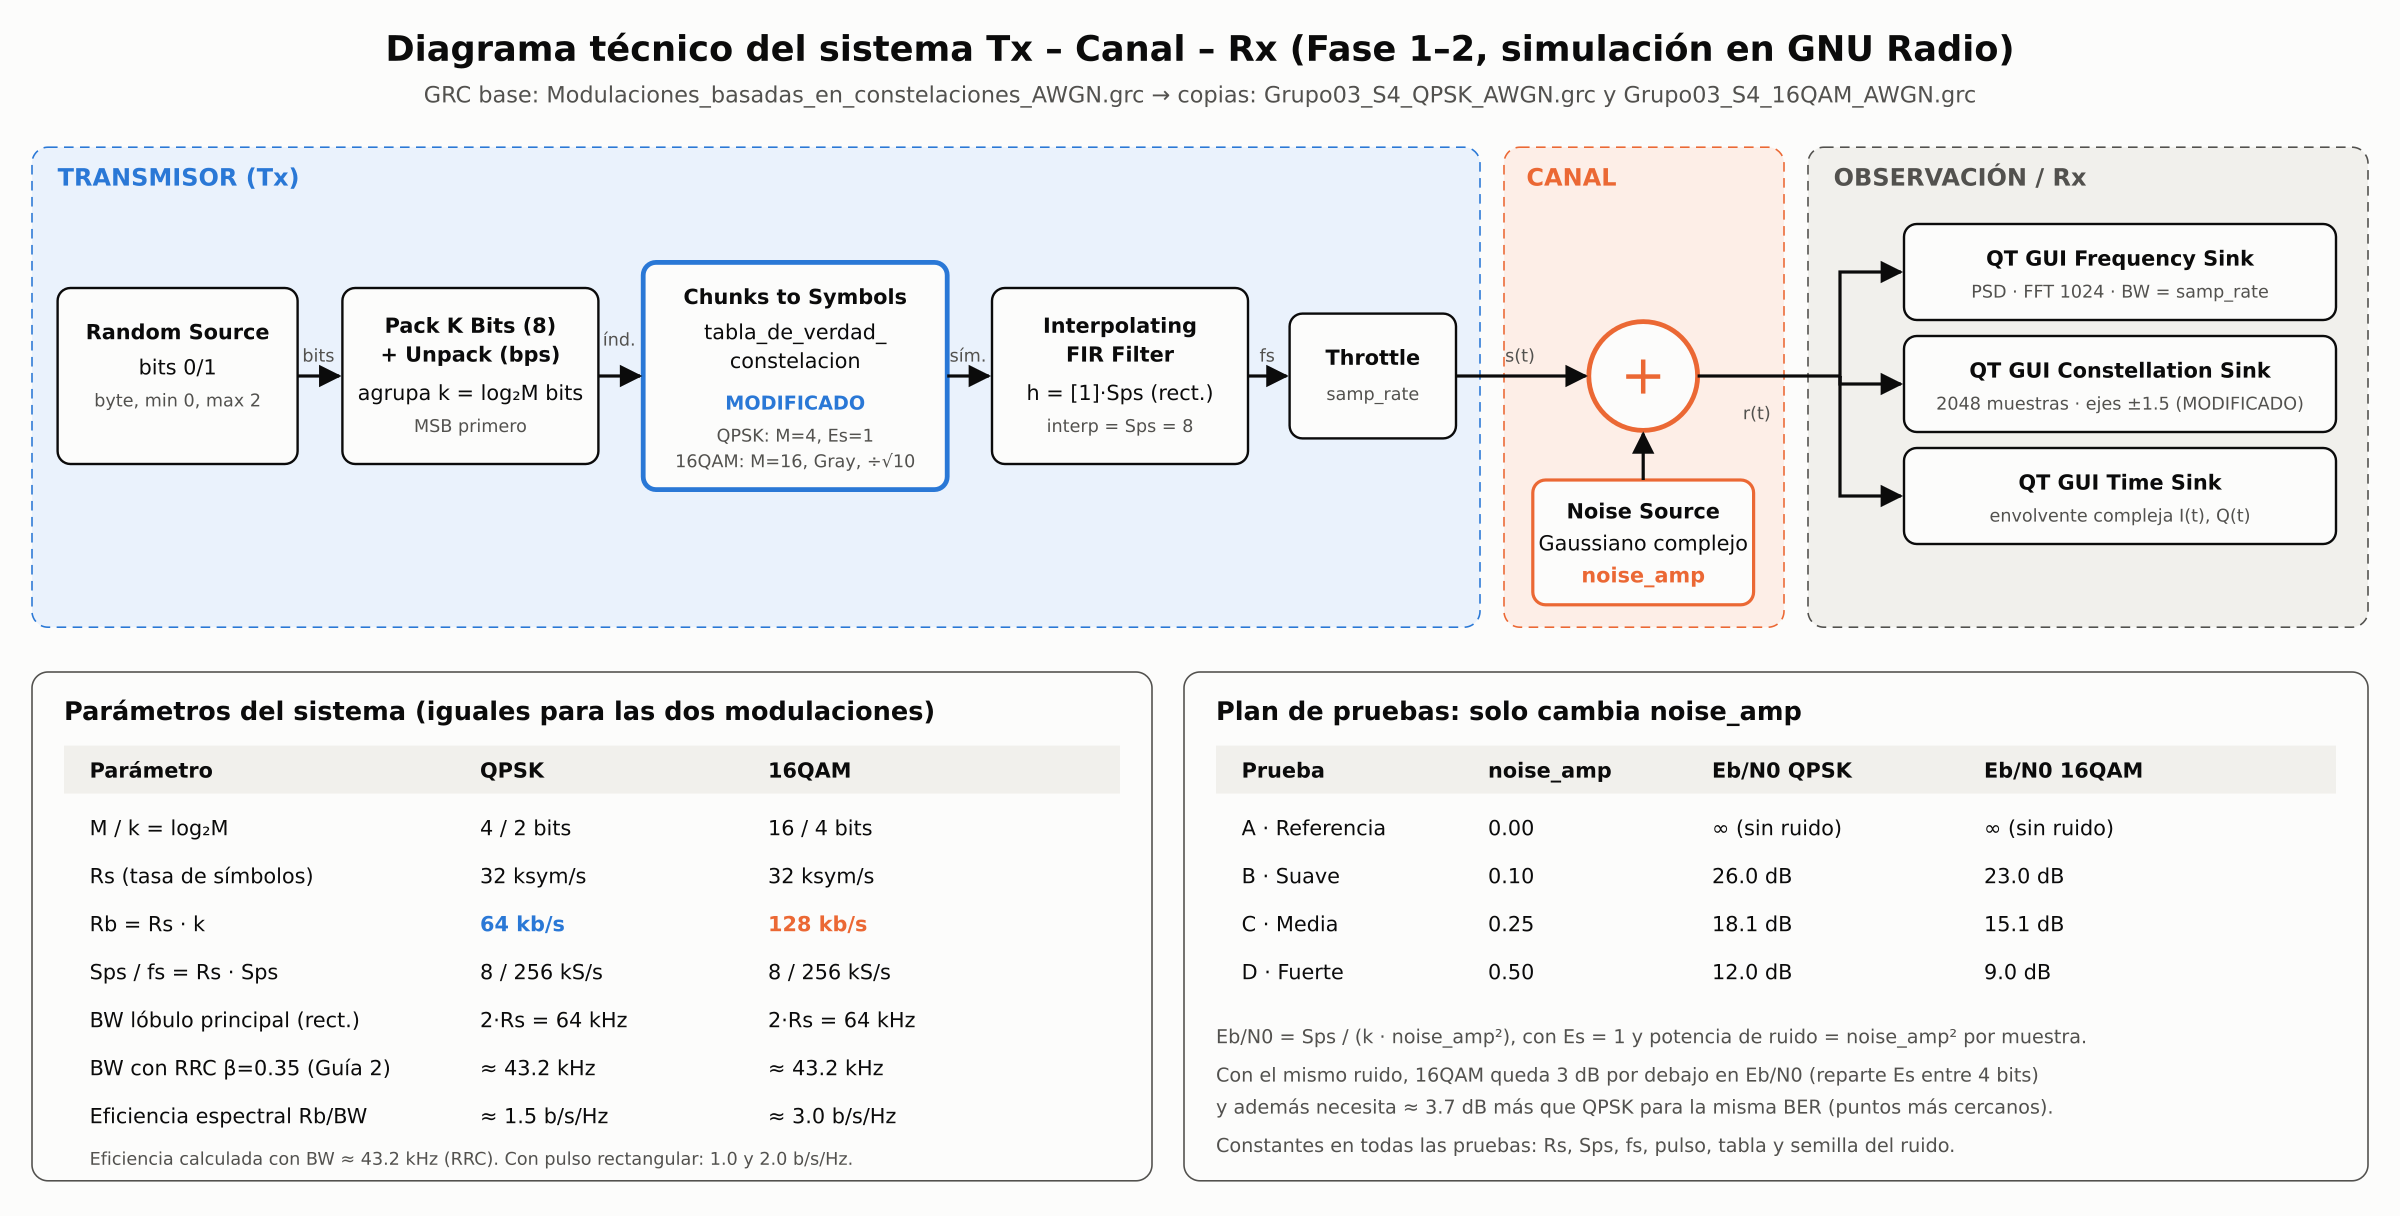
\includegraphics[width=0.95\textwidth]{diagramas_tecnicos/fig2_diagrama_bloques_Tx_canal_Rx.png}
\caption{Diagrama técnico del sistema Tx--canal--Rx, con los bloques del GRC, los parámetros y el plan de pruebas. El único bloque modificado en la cadena es la tabla de la constelación.}
\label{fig:bloques}
\end{figure*}

\section{Metodología de simulación en GNU Radio}
Se usó GNU Radio Companion 3.10 \cite{gnuradio}. Se conservó el archivo original \texttt{Modulaciones\_basadas\_en\_constelaciones\_AWGN.grc} y se trabajó sobre dos copias: \texttt{Grupo03\_S4\_QPSK\_AWGN.grc} y \texttt{Grupo03\_S4\_16QAM\_AWGN.grc}. Los cambios fueron pocos y todos están documentados en el repositorio: la tabla de la constelación (QPSK, o 16QAM Gray dividida entre $\sqrt{10}$), el valor inicial de \texttt{noise\_amp} en cero y los ejes de la constelación fijos en $\pm1.5$, para que las capturas se pudieran comparar entre sí. Además, se organizaron los visores en una cuadrícula (\texttt{gui\_hint}) para ver en una sola ventana la envolvente, la PSD y la constelación. La Fig.~\ref{fig:grc} muestra el flujograma de 16QAM tal como quedó en GNU Radio Companion 3.10 (radioconda, Windows), con $M=16$, \texttt{bps}~$=4$ y $R_b=128$k calculados automáticamente a partir de la tabla.

\begin{figure*}[!t]
\centering
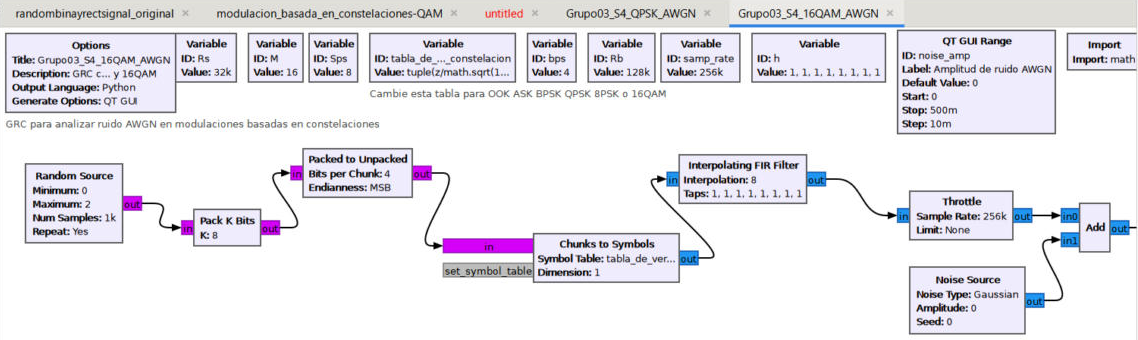
\includegraphics[width=0.9\textwidth]{capturas_gnuradio/grc_16QAM_flujograma.png}
\caption{Flujograma \texttt{Grupo03\_S4\_16QAM\_AWGN.grc} en GNU Radio Companion. Las variables $M$, \texttt{bps}, $R_b$ y \texttt{samp\_rate} se calculan a partir de la tabla de la constelación.}
\label{fig:grc}
\end{figure*}

Siguiendo la guía, se cambió una sola variable a la vez. Cada flujograma se ejecutó en GNU Radio y, con la ventana abierta, se ajustó el control \texttt{noise\_amp} y se capturaron las gráficas. Se hicieron cuatro pruebas por modulación, con el mismo \texttt{noise\_amp} para las dos: referencia (0), suave (0.10), media (0.25) y fuerte (0.50). Como el bloque de ruido entrega una potencia total $\sigma^2=\texttt{noise\_amp}^2$ por muestra y la señal tiene $E_s=1$, la relación por bit después de un filtro acoplado es
\begin{equation}
\frac{E_b}{N_0}=\frac{S_{ps}}{k\cdot\texttt{noise\_amp}^2}.
\end{equation}

El flujograma base no tiene receptor, así que para cuantificar lo que se ve en las constelaciones se reprodujo la misma cadena en Python (\texttt{scripts/sim\_fase1.py}). Allí se agregó un receptor ideal que integra las 8 muestras de cada símbolo (filtro acoplado para pulso rectangular) y decide por mínima distancia. Con él se midió la BER usando 400\,000 bits en QPSK y 800\,000 en 16QAM por prueba.

\section{Resultados}
\subsection{Constelaciones}
La Fig.~\ref{fig:const} reúne las ocho constelaciones capturadas en GNU Radio. En la referencia aparecen los puntos ideales. Con ruido suave, cada punto se vuelve una nube pequeña y todas siguen separadas. En la prueba media, las nubes de QPSK siguen bien definidas, mientras que en 16QAM ya empiezan a tocarse. De hecho, en la captura de 16QAM con ruido medio ya casi no se distinguen las 16 nubes a simple vista. Con ruido fuerte, QPSK todavía deja ver sus cuatro grupos, mientras que la constelación de 16QAM se vuelve una mancha uniforme.

\begin{figure*}[!t]
\centering
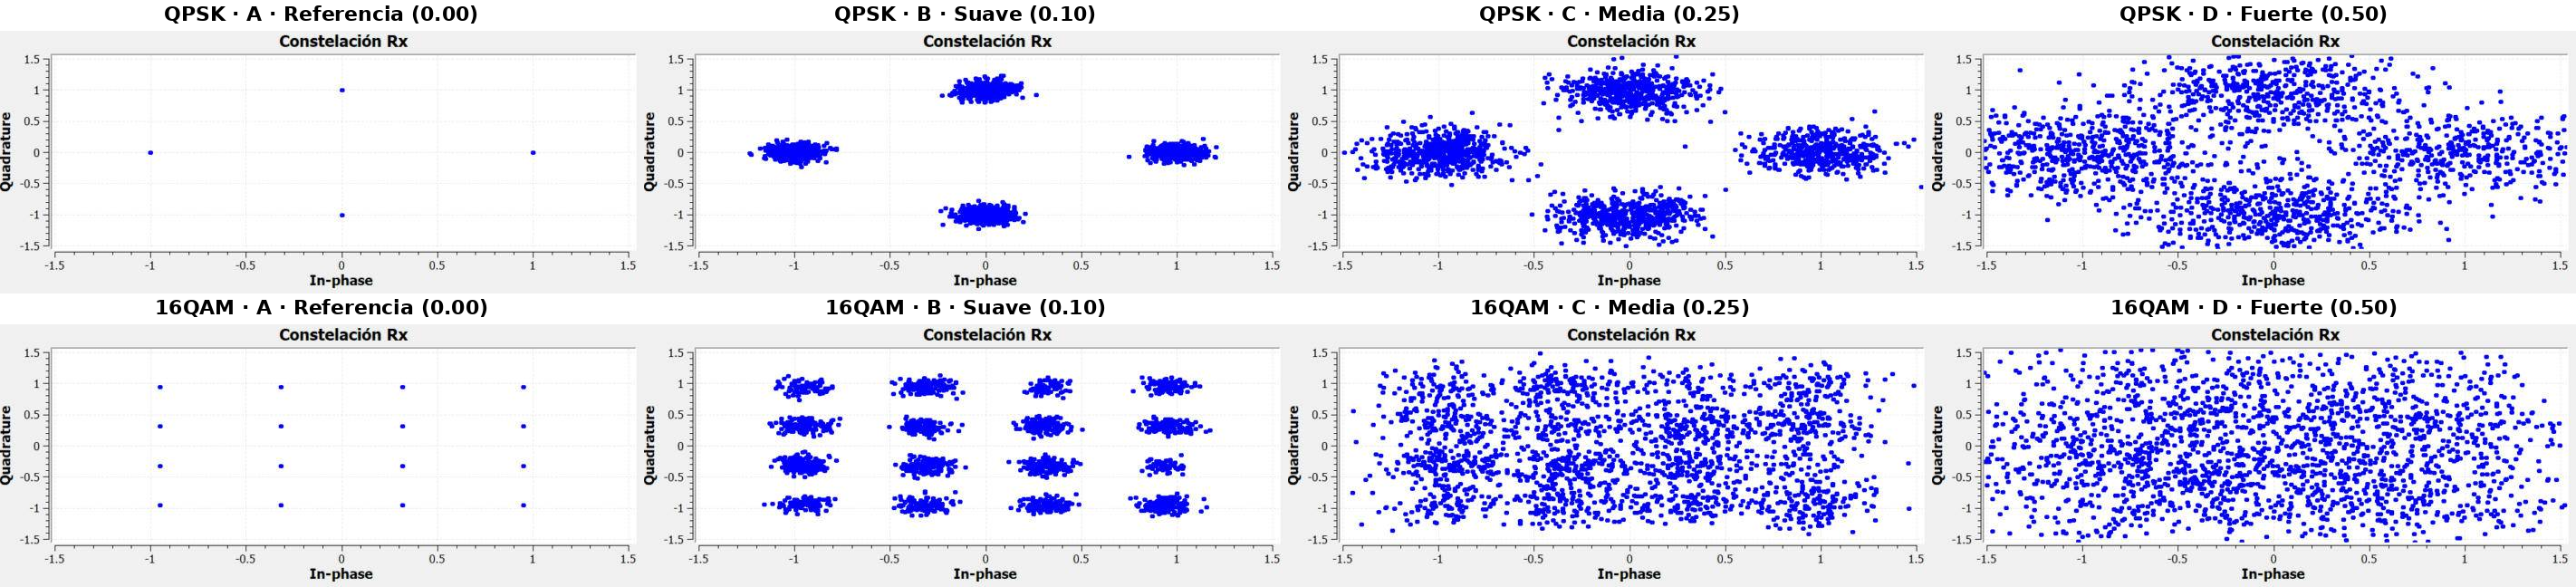
\includegraphics[width=\textwidth]{capturas_gnuradio/grc_constelaciones_QPSK_vs_16QAM_4pruebas.png}
\caption{Capturas del \emph{QT GUI Constellation Sink} en GNU Radio para QPSK (arriba) y 16QAM (abajo) en las cuatro pruebas; entre paréntesis, el valor de \texttt{noise\_amp}.}
\label{fig:const}
\end{figure*}

\subsection{Densidad espectral de potencia}
En la Fig.~\ref{fig:psd}, las PSD de QPSK y 16QAM tienen prácticamente la misma forma en las cuatro pruebas. En la referencia, las dos muestran el lóbulo principal entre $-32$ y $+32$~kHz (es decir, $2R_s=64$~kHz) y nulos en múltiplos de $R_s$ ($\pm32$, $\pm64$ y $\pm96$~kHz), que es la forma típica del pulso rectangular. Al aumentar el ruido, el lóbulo principal no se mueve ni se ensancha, pero el piso espectral sube y los nulos desaparecen. En la prueba fuerte, el piso queda cerca de $-40$~dB, apenas unos 20~dB por debajo del pico. Como el visor no promedia, las curvas se ven rugosas, pero la tendencia es clara.

\begin{figure*}[!t]
\centering
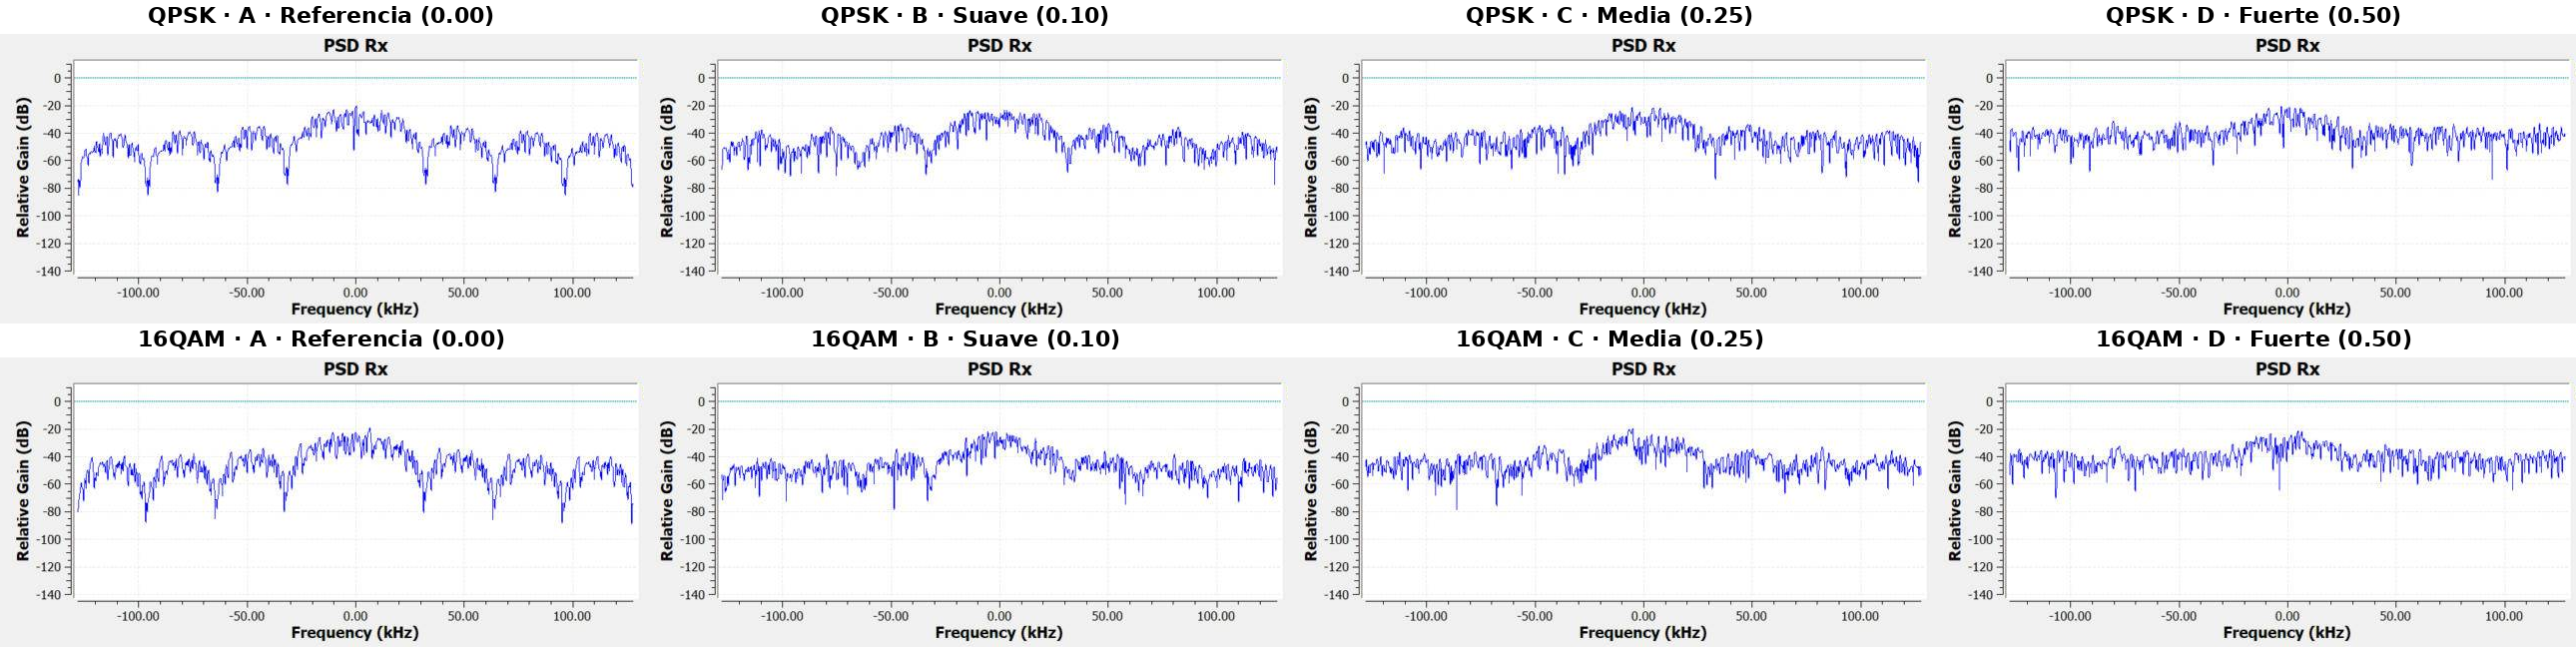
\includegraphics[width=\textwidth]{capturas_gnuradio/grc_PSD_QPSK_vs_16QAM_4pruebas.png}
\caption{Capturas del \emph{QT GUI Frequency Sink} (PSD) en GNU Radio para QPSK (arriba) y 16QAM (abajo). Las dos ocupan el mismo ancho de banda; el ruido solo eleva el piso espectral.}
\label{fig:psd}
\end{figure*}

\subsection{Señal temporal}
La Fig.~\ref{fig:tiempo} muestra 8~ms de la envolvente compleja (256 símbolos). En QPSK, cada símbolo pone la señal sobre un solo eje (I o Q vale $\pm1$ y el otro vale 0), mientras que en 16QAM cada componente toma uno de cuatro niveles ($\pm0.32$ y $\pm0.95$). Con ruido medio, en QPSK todavía se distinguen los niveles con facilidad, pero en 16QAM los niveles internos y externos quedan separados por solo 0.63 y ya son difíciles de reconocer a simple vista.

\begin{figure*}[!t]
\centering
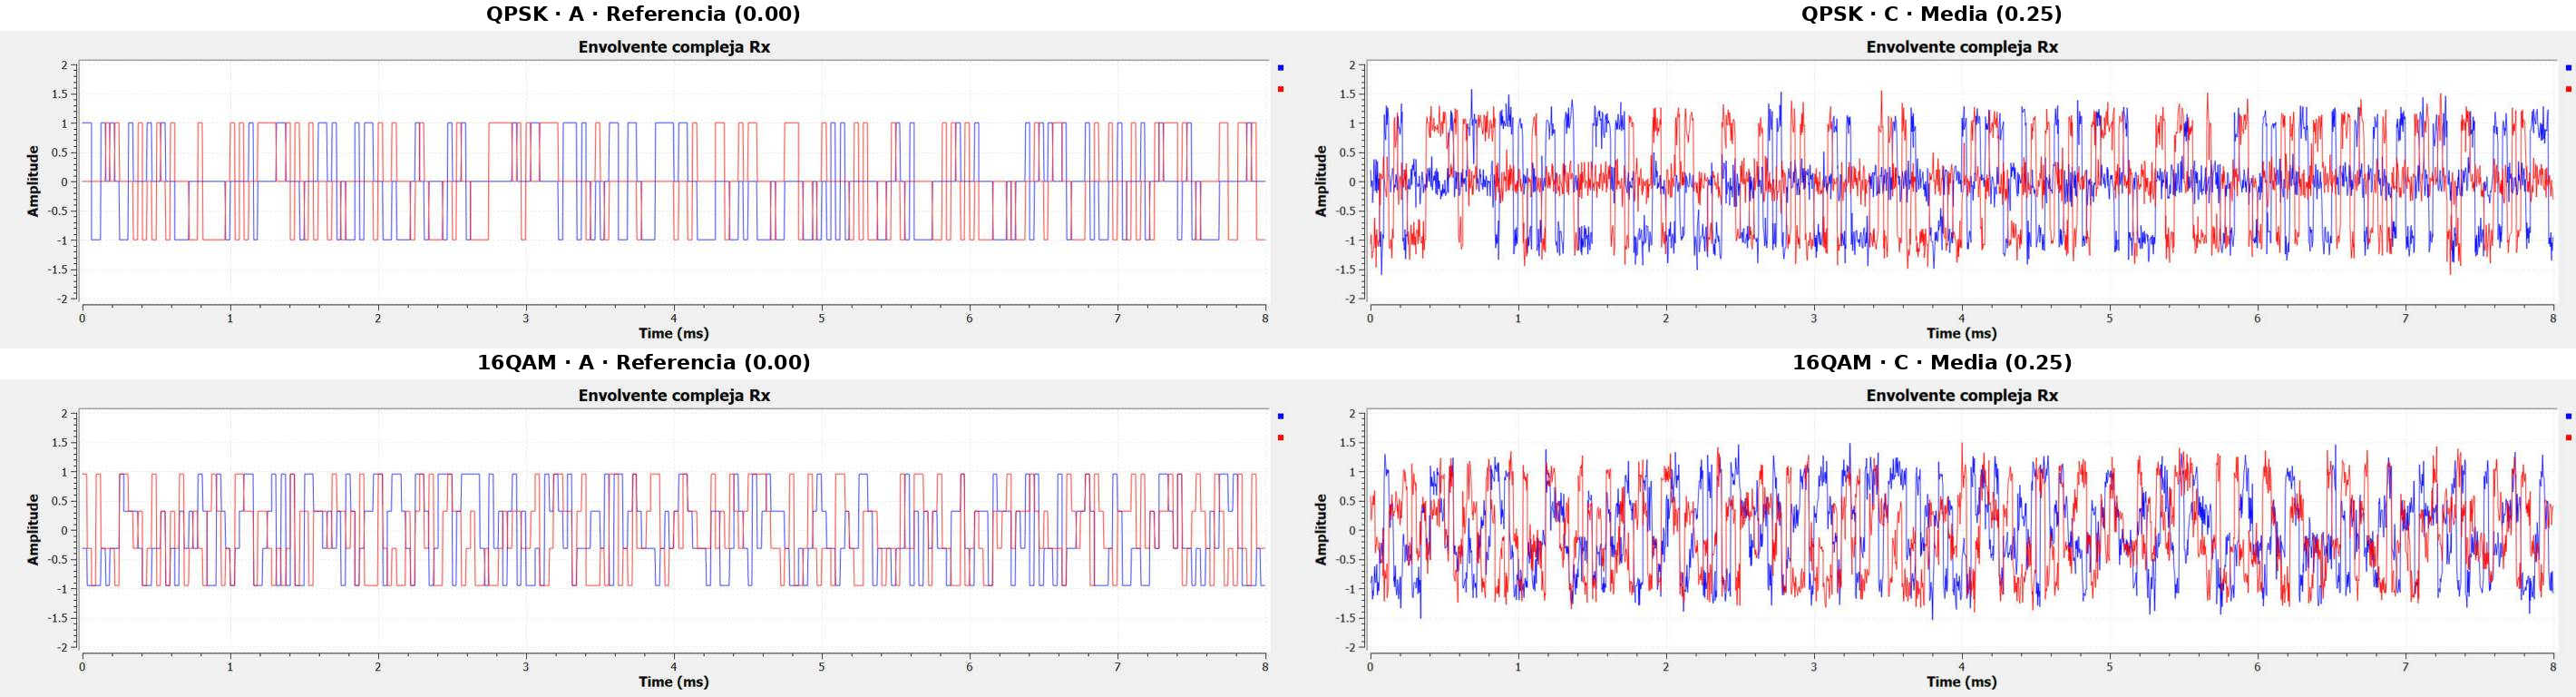
\includegraphics[width=\textwidth]{capturas_gnuradio/grc_envolvente_QPSK_vs_16QAM_AyC.png}
\caption{Capturas del \emph{QT GUI Time Sink} (envolvente compleja I(t) en azul y Q(t) en rojo, 8~ms) para QPSK y 16QAM en las pruebas A y C.}
\label{fig:tiempo}
\end{figure*}

\subsection{Tasa de error}
La Tabla~\ref{tab:pruebas} resume las pruebas. Hasta la prueba media, ninguna de las dos modulaciones tuvo errores con el receptor ideal. En la prueba fuerte, 16QAM ($E_b/N_0=9.0$~dB) tuvo una BER de $4.25\times10^{-3}$, muy cerca del valor teórico de $4.29\times10^{-3}$. QPSK, en cambio, con 12.0~dB, no tuvo ningún error en 400\,000 bits, lo cual concuerda con su BER teórica de $7.7\times10^{-9}$. La Fig.~\ref{fig:ber} compara las curvas teóricas con los puntos simulados.

\begin{table}[!t]
\caption{Pruebas realizadas (solo cambia \texttt{noise\_amp})}
\label{tab:pruebas}
\centering\footnotesize
\setlength{\tabcolsep}{3.5pt}
\begin{tabular}{@{}lccccc@{}}
\toprule
 & & \multicolumn{2}{c}{QPSK} & \multicolumn{2}{c}{16QAM}\\
\cmidrule(lr){3-4}\cmidrule(l){5-6}
Prueba & \texttt{noise\_amp} & $E_b/N_0$ & BER & $E_b/N_0$ & BER\\
\midrule
A Referencia & 0.00 & $\infty$ & 0 & $\infty$ & 0\\
B Suave & 0.10 & 26.0 dB & 0 & 23.0 dB & 0\\
C Media & 0.25 & 18.1 dB & 0 & 15.1 dB & 0\\
D Fuerte & 0.50 & 12.0 dB & 0 & 9.0 dB & $4.2\times10^{-3}$\\
\bottomrule
\end{tabular}
\end{table}

\begin{figure}[!t]
\centering
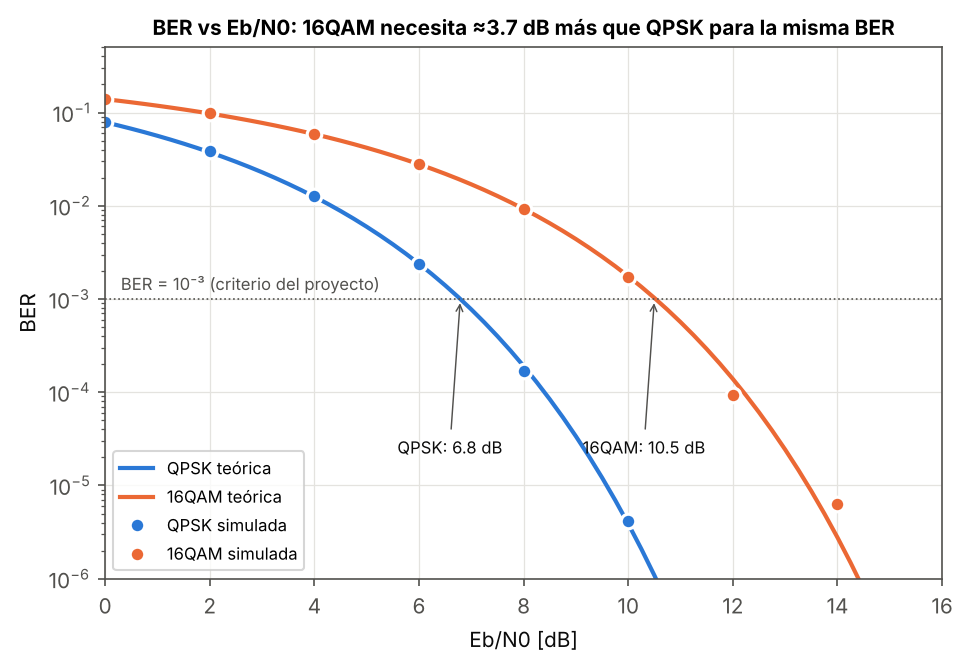
\includegraphics[width=\columnwidth]{diagramas_tecnicos/curva_BER_teorica_QPSK_vs_16QAM.png}
\caption{BER en función de $E_b/N_0$: curvas teóricas y puntos simulados con la misma cadena del GRC y un receptor de filtro acoplado.}
\label{fig:ber}
\end{figure}

\subsection{Validación en hardware}
El enlace 16QAM se llevó a hardware el 5 de noviembre de 2026, con los flujogramas \texttt{LAB\_TX/RX\_16QAM\_HackRF\_MEJORADO.grc} y dos HackRF One a 960~MHz, comunicados por antenas. Para que el radio recuperara el enlace de forma estable se usaron $R_s=8$~ksym/s, $S_{ps}=8$ (64~kS/s en banda base) y un filtro RRC con $\beta=0.5$. Esto da $R_b=32$~kb/s y un ancho de banda cercano a 12~kHz. El transmisor envía tramas conocidas (preámbulo, mensaje y CRC32), y el receptor sincroniza portadora y reloj, corrige las rotaciones de 90°, 180° y 270° de la constelación con el preámbulo y calcula la BER y el EVM.

En la mejor condición se obtuvo una BER acumulada cercana al 0.34\,\%, un EVM de 7.4\,\% y el 81\,\% de las tramas con CRC correcto (Fig.~\ref{fig:lab}).

\begin{figure}[!t]
\centering
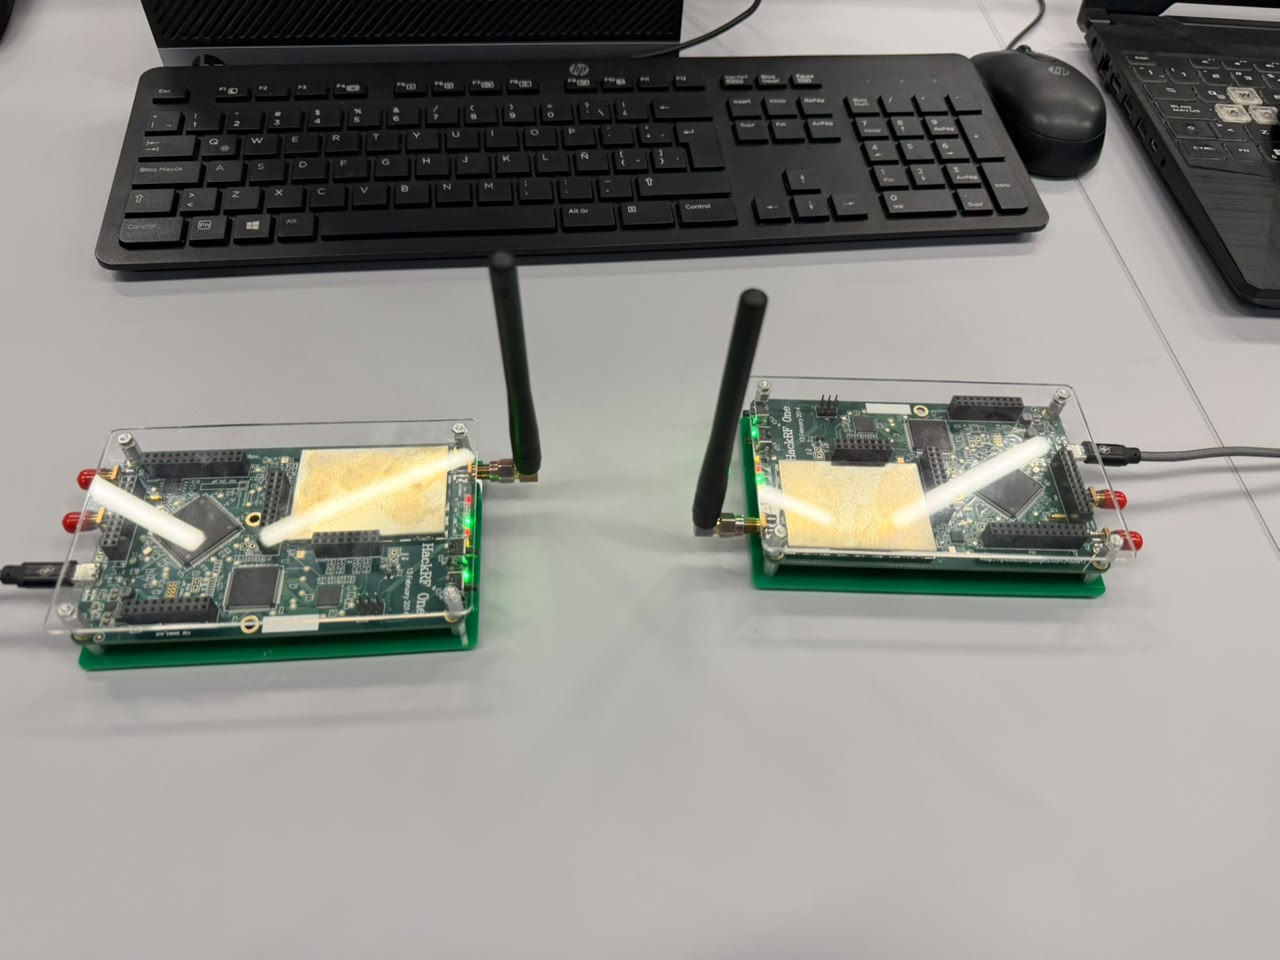
\includegraphics[width=0.49\columnwidth]{evidencias_laboratorio/lab_2026-11-05_01.jpg}\hfill
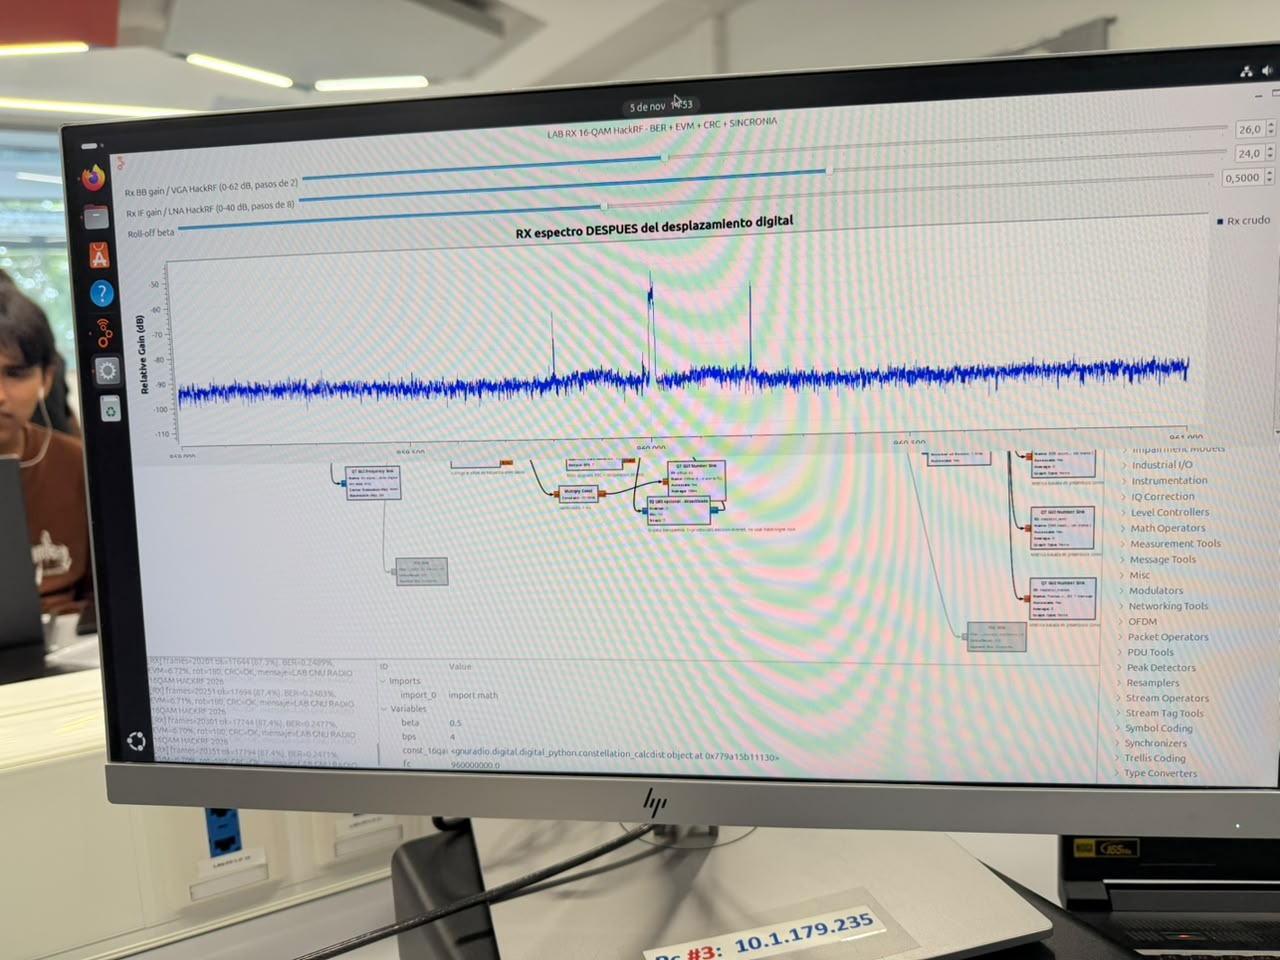
\includegraphics[width=0.49\columnwidth]{evidencias_laboratorio/lab_2026-11-05_02.jpg}
\caption{Evidencias del laboratorio con HackRF One: a la izquierda, los dos radios con sus antenas; a la derecha, el espectro recibido después del desplazamiento digital.}
\label{fig:lab}
\end{figure}

\section{Análisis de resultados}
Los resultados confirman la hipótesis de la ficha de decisión. En primer lugar, el ancho de banda no cambió al pasar de QPSK a 16QAM: las PSD son prácticamente iguales porque las dos usan la misma $R_s$ y el mismo pulso. Sin embargo, 16QAM transportó el doble de bits, así que su eficiencia espectral también se duplicó. Este es el beneficio que busca el escenario S4.

En segundo lugar, con el mismo ruido, 16QAM se degradó antes. Hay dos razones que se suman. La primera es geométrica: como sus puntos están 2.2 veces más cerca, una misma nube de ruido alcanza a cruzar la frontera de decisión con mucha más facilidad. La segunda es energética: con la misma $E_s$ y el mismo ruido, 16QAM reparte la energía de cada símbolo entre 4 bits en lugar de 2, así que su $E_b/N_0$ queda 3~dB por debajo de la de QPSK, como se ve en la Tabla~\ref{tab:pruebas}.

Vale la pena aclarar algo sobre las constelaciones del GRC. El visor dibuja todas las muestras, sin pasar por un filtro acoplado. Por eso la relación señal a ruido que se ve en la Fig.~\ref{fig:const} es $1/\texttt{noise\_amp}^2$ por muestra, y no $S_{ps}/\texttt{noise\_amp}^2$, que es la que tiene un receptor real. Esa diferencia, de unos 9~dB, explica por qué la constelación de 16QAM en la prueba media se ve bastante sucia y aun así el receptor ideal no tuvo errores: al integrar las 8 muestras de cada símbolo, gran parte del ruido se cancela. Este resultado justifica el filtro acoplado que pide la Guía~2.

Por último, en hardware la BER de 0.34\,\% (cerca de $3.4\times10^{-3}$) apareció sin añadir ruido artificial. Esto indica que el enlace real ya tiene sus propias imperfecciones: ruido del receptor, desfase de frecuencia entre los dos radios, multitrayectoria en el laboratorio e interferencia de otros grupos que transmitían cerca. De hecho, en una de las capturas el receptor decodificó un mensaje distinto al esperado, con una BER cercana al 29\,\%, lo que sugiere que se enganchó a la señal de otro equipo. Aquí se ve la importancia del preámbulo y del CRC para validar cada trama.

\section{Conclusiones y trabajo futuro}
Con la misma tasa de símbolos, 16QAM duplica la tasa de bits sin ocupar más espectro. En nuestra simulación pasó de 64~kb/s a 128~kb/s dentro del mismo lóbulo de 64~kHz. La capacidad extra se paga con robustez: con la misma potencia y el mismo ruido, 16QAM falló en la prueba fuerte, mientras que QPSK no tuvo errores, y por teoría necesita unos 3.7~dB más de $E_b/N_0$ para la misma BER.

Para la aplicación del escenario, 16QAM es la mejor opción cuando el enlace tiene buena relación señal a ruido, como un enlace corto y con línea de vista dentro de la planta. Si el canal se vuelve ruidoso, QPSK es más segura. La solución más completa sería adaptar la modulación según la calidad del enlace.

Como trabajo futuro se propone completar la medición de la curva BER vs $E_b/N_0$ en hardware con el instrumento de la Fase~4, idealmente por cable y con atenuadores, para compararla con la curva teórica en BER $=10^{-3}$. También se propone repetir la simulación con el filtro RRC de la Guía~2 y un receptor completo con sincronización.

\begin{thebibliography}{9}
\footnotesize
\bibitem{proakis} J. G. Proakis and M. Salehi, \emph{Digital Communications}, 5th ed. New York, NY, USA: McGraw-Hill, 2008.
\bibitem{sklar} B. Sklar, \emph{Digital Communications: Fundamentals and Applications}, 2nd ed. Upper Saddle River, NJ, USA: Prentice Hall, 2001.
\bibitem{goldsmith} A. Goldsmith, \emph{Wireless Communications}. Cambridge, U.K.: Cambridge Univ. Press, 2005.
\bibitem{haykin} S. Haykin, \emph{Communication Systems}, 5th ed. Hoboken, NJ, USA: Wiley, 2009.
\bibitem{gnuradio} GNU Radio Project, ``GNU Radio Companion,'' GNU Radio Wiki. [Online]. Available: https://wiki.gnuradio.org
\bibitem{guia} O. Tíjaro and R. Zamora, ``Proyecto Integrador de Comunicaciones II: Guía del estudiante,'' Universidad Industrial de Santander, Bucaramanga, Colombia, 2026.
\end{thebibliography}

\end{document}
